\documentclass[conference]{IEEEtran}

\usepackage{listings}
\usepackage{pgfplots}
\pgfplotsset{compat=1.6}
\usepackage{hyperref}
\usepackage{caption}
\usepackage{subcaption}
\usepackage{tikz}

\usepackage[
  backend=biber,
  style=ieee,
  sorting=none
]{biblatex}
\addbibresource{CAD.bib}

\lstset{basicstyle=\footnotesize\ttfamily,
  breaklines=true}




\begin{document}

\title{Performance enhancement using MPI in a simulation of heat diffusion}

\author{
  \IEEEauthorblockN{Gonçalo Lourenço \\ nº55780 \\ gm.lourenco@campus.fct.unl.pt}
  \and
  \IEEEauthorblockN{Joana Faria \\ nº55754 \\ js.faria@campus.fct.unl.pt}
}

\maketitle



\section{Introduction}
This assignment aims to optimize a base code, written in \texttt{C}, that computes a simulation for heat diffusion. This time we intend to parallelize the computation using the Message Passing Interface (MPI).

To find the best performance we will explore different approaches, namely analyzing different patterns of communication and trying to overlap the communication with the computation.

We have available, for this assignment, two nodes, each one with 16 true CPUs.\@ Given this information, we can have a maximum of 32 processes.


\section{Results}
We experiment with many versions of a parallel program using MPI, these versions are explained and analyzed below.

To establish a baseline for comparison we start by analyzing the execution time of the sequential version and we obtain an average of 153.979 seconds, with the following parameters:
\begin{verbatim}
  // Width of the area
  const int nx = 200;
  // Height of the area
  const int ny = 200;
  // Diffusion constant           
  const float a = 0.5;
  // h=dx=dy  grid spacing
  const float h = 0.005;
  // Number of time steps to simulate
  const int numSteps = 100000;  
  // How frequently to write output image
  const int outputEvery = 100000;
\end{verbatim}

Unless otherwise stated, these will be the parameters used for determining the execution times.

\section{Discussion}

\subsection{V1 version --- Synchronous Communication}\label{sec:v1}

In version V1 we start with a simple parallel version where we distribute the lines of the original matrix by the number of processes and perform synchronous communication between neighbors processes to obtain the border necessary for the computation.

For the communication necessary to write the output we use the \texttt{MPI\_Send} and \texttt{MPI\_Recv} methods, where all process sends their results to process 0, which aggregates all the results and writes the output file.

In \autoref{fig:executionTimeV1} we can see the execution time for V1, comparing the performance of this version for different numbers of processes. From this graphic we can see the bigger improvement until 16 processes, these processes run on the same machine. For the sake of completeness, we test with 17 processes and we can observe a slight worsening, this is because only one process is running on a different machine, adding communication overhead. Is due to this communication overhead that the improvements aren't bigger when we use 32 or 48 processes.

\begin{figure}[ht]
  \centering
  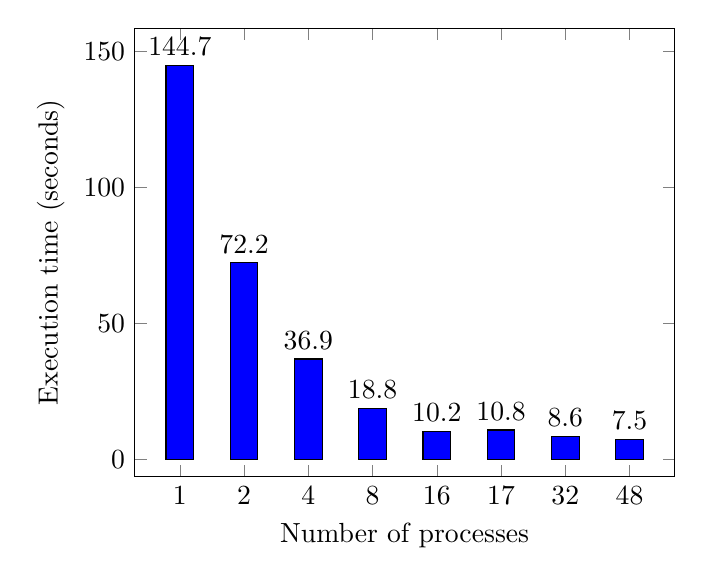
\begin{tikzpicture}

    \begin{axis}[
        ylabel={Execution time (seconds)},
        xlabel={Number of processes},
        symbolic x coords={1,2, 4, 8, 16, 17, 32, 48},
        xtick=data,
        nodes near coords={
            \pgfmathprintnumber[precision=1]{\pgfplotspointmeta}
          },
      ]
      \addplot[ybar,fill=blue] coordinates {
          (1,   144.74)
          (2,   72.22)
          (4,  36.92)
          (8,   18.83)
          (16,   10.23)
          (17,   10.83)
          (32,   8.57)
          (48,   7.45)
        };
    \end{axis}
  \end{tikzpicture}
  \caption{Execution time of V1 varying the number of processes}
  \label{fig:executionTimeV1}
\end{figure}

\subsection{V2 --- Gather}\label{sec:v2}
In this version, we modify version V1 to use the method \texttt{MPI\_Gather} for the phase of writing the output. The results are similar to version V1, and are presented in \autoref{fig:executionTimeV2}.


\begin{figure}[ht]
  \centering
  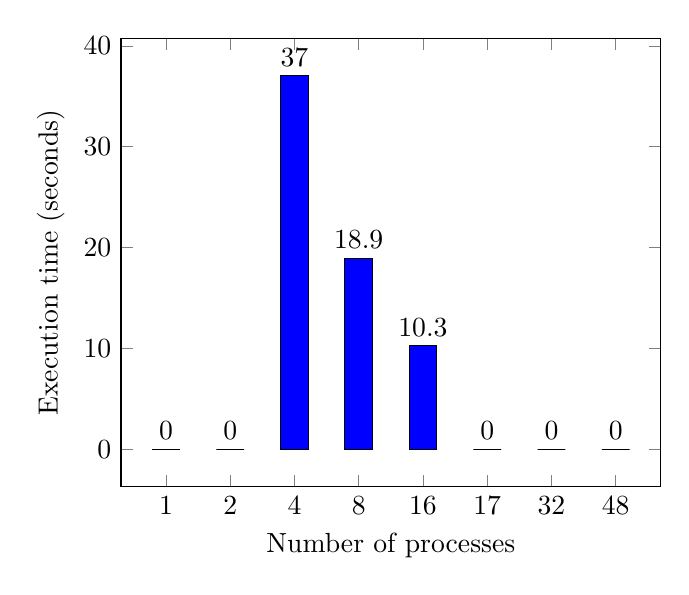
\begin{tikzpicture}

    \begin{axis}[
        ylabel={Execution time (seconds)},
        xlabel={Number of processes},
        symbolic x coords={1,2, 4, 8, 16, 17, 32, 48},
        xtick=data,
        nodes near coords={
            \pgfmathprintnumber[precision=1]{\pgfplotspointmeta}
          },
      ]
      \addplot[ybar,fill=blue] coordinates {
          (1,   0)
          (2,   0)
          (4,  37.03)
          (8,   18.91)
          (16,   10.26)
          (17,   0)
          (32,   0)
          (48,   0)
        };
    \end{axis}
  \end{tikzpicture}
  \caption{Execution time of V2 varying the number of processes}
  \label{fig:executionTimeV2}
\end{figure}

\subsection{V3 --- One node for output}
In V3 we assign node 0 the function of joining the output of all the other nodes, performing no computation concerning the heat equation. This version was intended as a first step to overlap computation with communication in situations where output is stored more frequently. In this version, we keep synchronous communication.


\section{Compilation and Execution Instructions}
Our best version, V2, can be compiled and executed with the following command, from inside the folder \texttt{/proj1}:
\begin{verbatim}
nvcc -o v2 v2.cu && ./v2
\end{verbatim}
This will execute ten iterations to measure the average execution times and the results of the heat equation will be saved in the folder \texttt{images/v2}.


\printbibliography


\end{document}